\documentclass[t]{beamer}
\usepackage{susu}

\begin{document}
	
	\firstpage
	\justifying
\section{Введение}
	\begin{frame}
		\begin{figure}
			\centering
			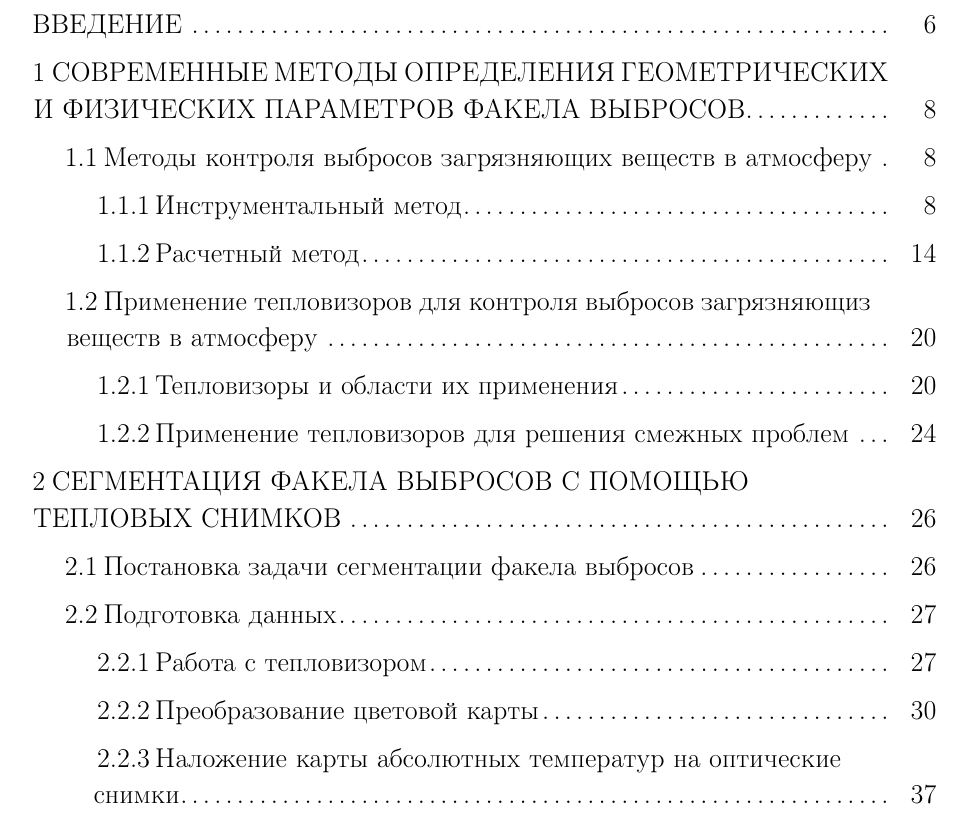
\includegraphics[width = 7cm]{image/ToC}
			\caption{Оглавление}
		\end{figure}
	\end{frame}

	\begin{frame}
		\frametitle{\insertsection} 
		В современном мире остро возникла проблема загрязнения воздуха. Выбросы заводов и автомобилей приводят к повышению температуры воздуха и загрязнению атмосферы химическими соединениями. Решением этой проблемы является сокращение количества выбросов в атмосферу вредных соединений промышленными предприятиями. На сегодняшний день эта проблема решается с помощью контроля за содержанием и объемом дыма. Многие геометрические и физические характеристики выбросов можно проанализировать, используя тепловые и оптические снимки. Для реализации подобного способа анализа можно воспользоваться классическими методами компьютерного зрения.
	\end{frame}

	\begin{frame}
		Целью данной работы является расчет геометрических и физических свойств выбросов предприятий. Для достижения данной цели необходимо решить следующие задачи:
		\begin{enumerate}
			\justifying
			\item исследование существующих методов для решения задачи получения геометрических и физических характеристик выбросов;
			\item исследование современных способов применения оптических и тепловых снимков;
			\item разработка алгоритма для сегментации факела выбросов с использованием тепловых и оптических снимков;
			\item разработка алгоритма получения физических характеристик факела выбросов.
		\end{enumerate}
	\end{frame}

\section{Современные методы контроля выбросов}
	\begin{frame}
		\frametitle{\insertsection} 
		\bfseries Инструментальный метод \normalfont -- осуществление контроля с помощью газоаналитических средств. Особенности этого метода:
		\begin{enumerate}
			\justifying
			\item подходит для работы с организованными источниками;
			\item для реализации данного метода преимущественно используются газоанализаторы;
			\item высокая точность, что является преимуществом;
			\item сложность настройки и эксплуатации, высокая стоимость используемой аппаратуры, что явлеяется недостатком.
		\end{enumerate}
	\end{frame}
	
	\begin{frame}
		\bfseries Расчетный метод \normalfont используется для расчетов рассеивания выбросов от источников выброса загрязняющих атмосферный воздух веществ с помощью формул. Особенности этого метода:
		\begin{enumerate}
			\justifying
			\item менее точный, что является серьезным минусом;
			\item более дешевым в сравнении с инструментальным методом; 
			\item необходимость установки сложной и дорогой аппаратуры все еще есть, что делает этот метод все еще достаточно затратным;
		\end{enumerate}
		
		Решением данной проблемы может являтся использование тепло-видео систем наблюдения. Они значительно менее дорогие, чем газоанализаторы, при этом использование тепловых видео для сегментации и расчета объема выбросов позволит увеличить точность в сравнении с применением исключитьно оптических видео.
	\end{frame}

%	\begin{frame}
%		Где $A$ -- коэффициент, зависящий от температурной стратификации атмосферы;
%		$M$ -- масса ЗВ, выбрасываемого в атмосферный воздух в единицу времени, г/с;
%		$F$, $m$, $n$ и $\eta$ -- безразмерный коэффициенты;
%		$V_1$ -- расход ГВС, определяемый по формуле~(\ref{eq:V1}), м /с;
%		$\Delta T$ -- разность между температурой выбрасываемой ГВС $T_r$ и температурой атмосферного воздуха $T_B$, °С.
%		\begin{equation}
%			V_1 = \frac{\pi D^2}{4} \omega_0,
%			\label{eq:V1}
%		\end{equation}
%		где $D$ -- диаметр устья источника выброса, м;
%		$\omega_0$ -- средняя скорость выхода ГВС из устья источника выброса, м/с.
%		
%	\end{frame}

\section{Подготовка данных}

	\begin{frame}
		\frametitle{\insertsection} 
		Для решения поставленной задачи необходимо разработать алгоритм взаимодействия с тепловизором и научиться получать данные для последующей обработки. Подготовку данных можно разделить на три этапа:
		\begin{enumerate}
			\item работа с тепловизором;
			\item преобразование цветовой карты;
			\item наложение карты абсолютных температур на оптические снимки.
		\end{enumerate}
	\end{frame}


	\begin{frame}
		\bfseries Работа с тепловизором. \normalfont
		Для решения поставленной задачи был выбран тепловизор модели DS60xxFT-M. Для удаленной работы с ним былb предоставлены набор готовых программ с открытым исходным кодом и библиотека, содержащая реализации интерфейса для взаимоджействия с тепловизором. В возможности библиотеки входит:
		\begin{enumerate}
			\item управление положением тепловизора;
			\item получение матрицы температур;
			\item сохранение оптических и тепловых снимков покадрово в память компьютера в формате YUV.
		\end{enumerate}
	\end{frame}

	\begin{frame}
		При этом библиотека не позволяет получать матрицу абсолютных температур с частотой больше чем 1 Ггц, поэтому было решено записывать поток оптически и тепловых снимков с частотой 20 Ггц и максимальную и минимальную температуры с частотой в 1 Ггц, для преобразования относительных температур в абсолютные. Оптические и тепловые снимки записываются в формате YUV.
		\begin{figure}[ht!]
			\begin{subfigure}{.45\textwidth}
				\centering
				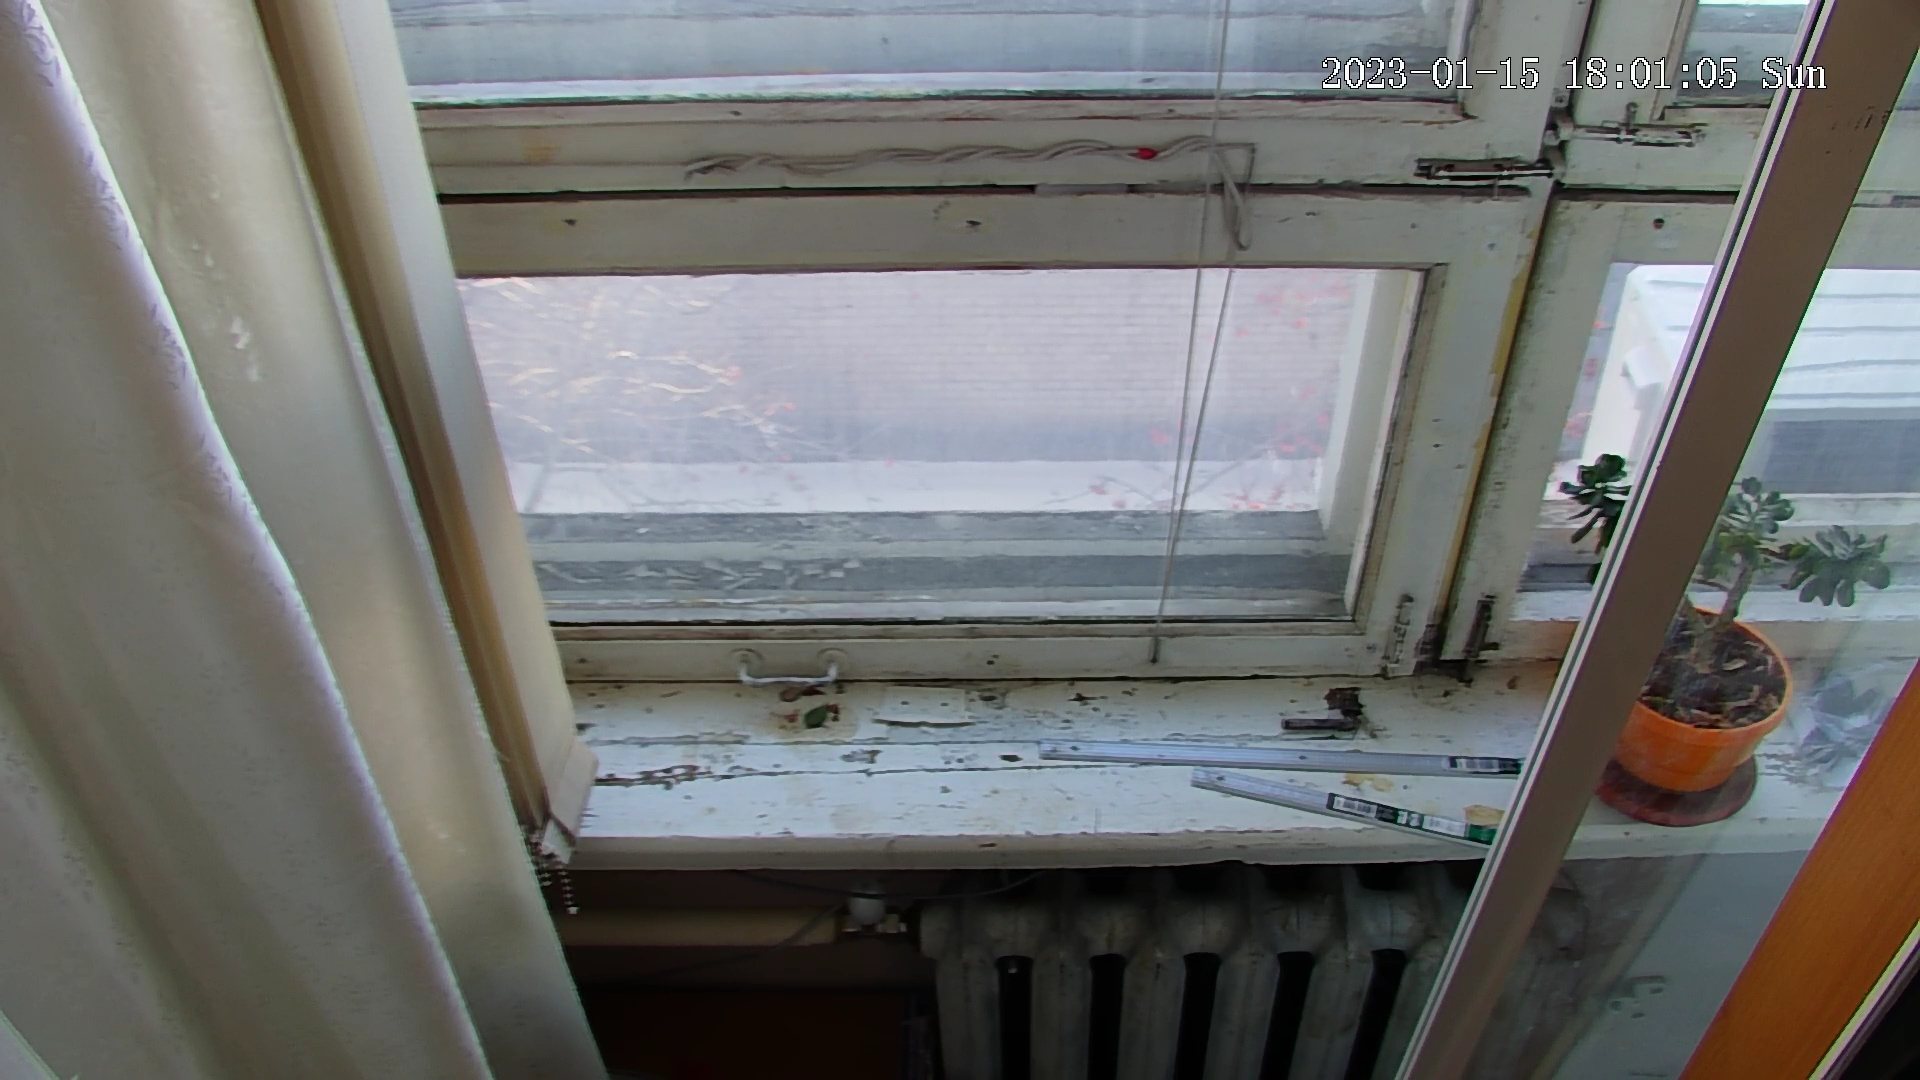
\includegraphics[width = 3cm]{image/chapter_2/opt_example}
				\caption{}
			\end{subfigure}
			\begin{subfigure}{.45\textwidth}
				\centering
				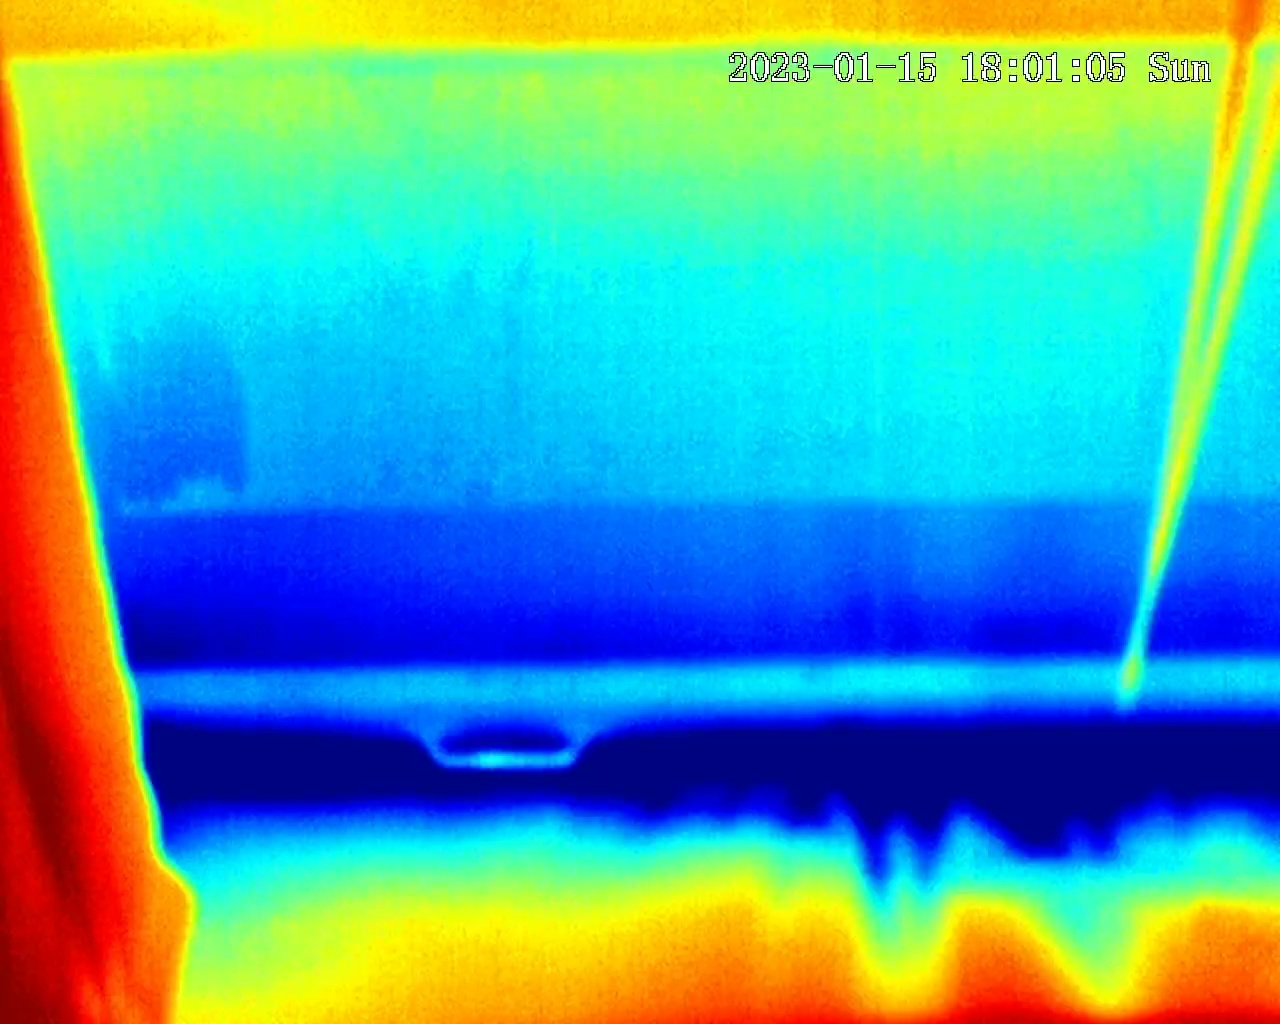
\includegraphics[width = 3cm]{image/chapter_2/tep_example}
				\caption{}
			\end{subfigure}
			\centering
			\caption{Примеры полученых изображений, где (a) оптический снимок; (б) тепловой снимок}
			\label{fig:Examples}
		\end{figure}
	\end{frame}

	\begin{frame}
		\bfseries Преобразование цветовой карты. \normalfont
		На рисунке~\ref{fig:Examples} видно, что тепловые снимки записываются с использованием цветовой карты. Цветовые карты необходимы для лучшего восприятия человеком изображения, при этом для автоматической обработки они не удобны. Поэтому возникает необходимость перевода теплового снимка в оттенки серого. В нашем случае была применена цветовая карта <<JET>> (рисунок \ref{fig:jet}).
		\begin{figure}[ht!]
			\centering
			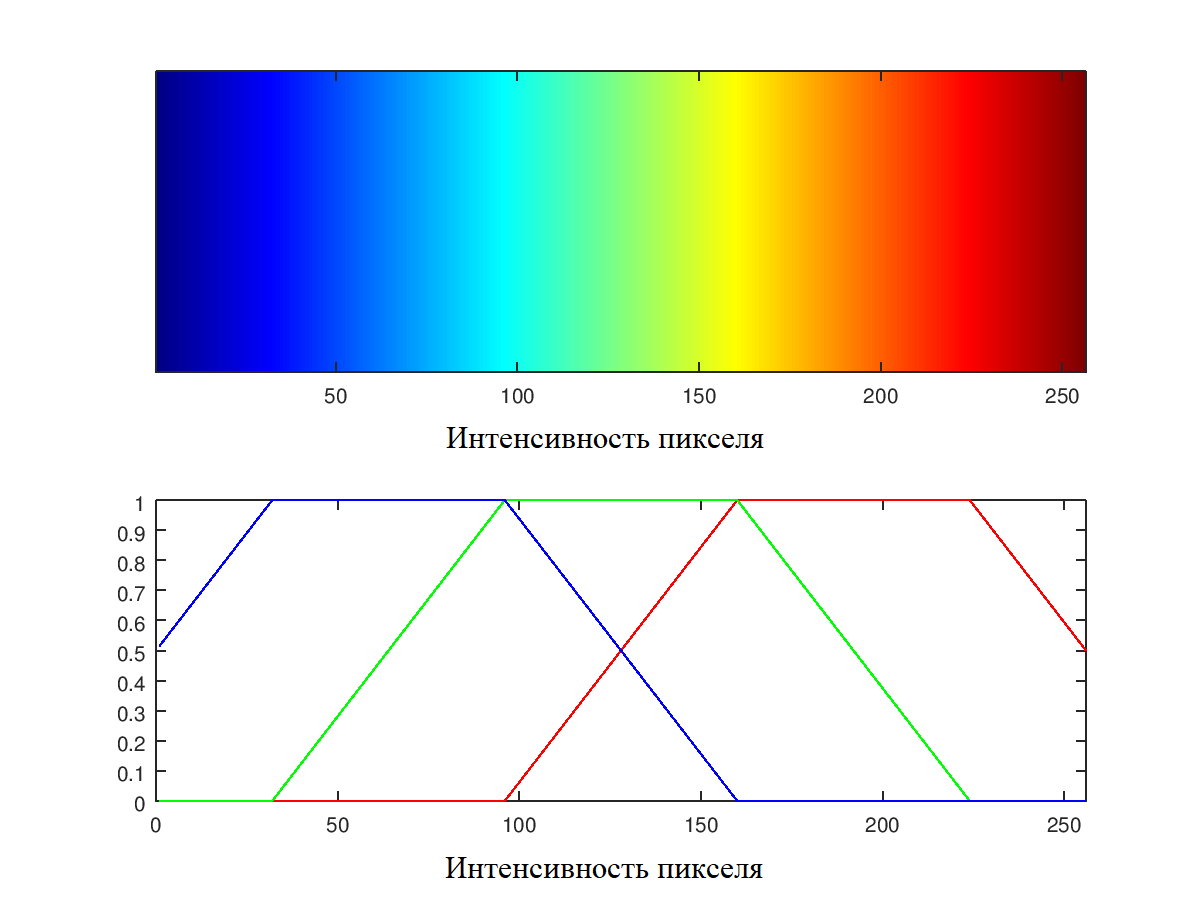
\includegraphics[width = 7cm]{image/chapter_2/jet}	
			\caption{График преобразования цвета в\\цветовой карте <<JET>>}
			\label{fig:jet}
		\end{figure}
	\end{frame}

	\begin{frame}
		Однако восстановить исходную функцию аналитически не представляется возможным, так как при передаче изображения используется технология сжатия JPEG и некоторые цвета изменяются. Для решения этой проблемы используется модель \\ <<FlannBasedMatcher>>. Эта модель работает на основе метода $k$-ближайших соседей, оптированного с помощью структуры данных <<$k$-мерное дерево>>.
		\begin{figure}[h!]
			\centering
			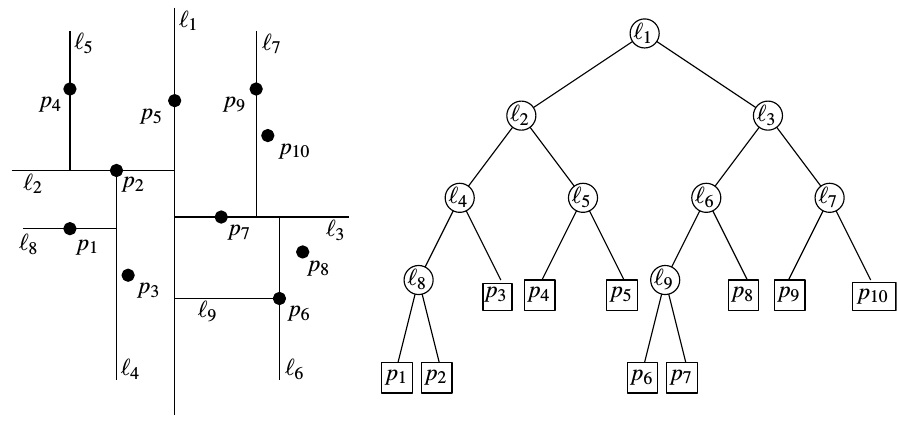
\includegraphics[width = 6cm]{image/chapter_2/kdtreeexample}	
			\caption{Пример построения k-мерного дерева}
			\label{fig:kdtreeexample}
		\end{figure}
		
	\end{frame}
	
	\begin{frame}
		Результат работы алгоритма преобразования можно увидеть на рисунке \ref{fig:ResKNN}.
		\begin{figure}[ht!]
			\begin{subfigure}{.45\textwidth}
				\centering
				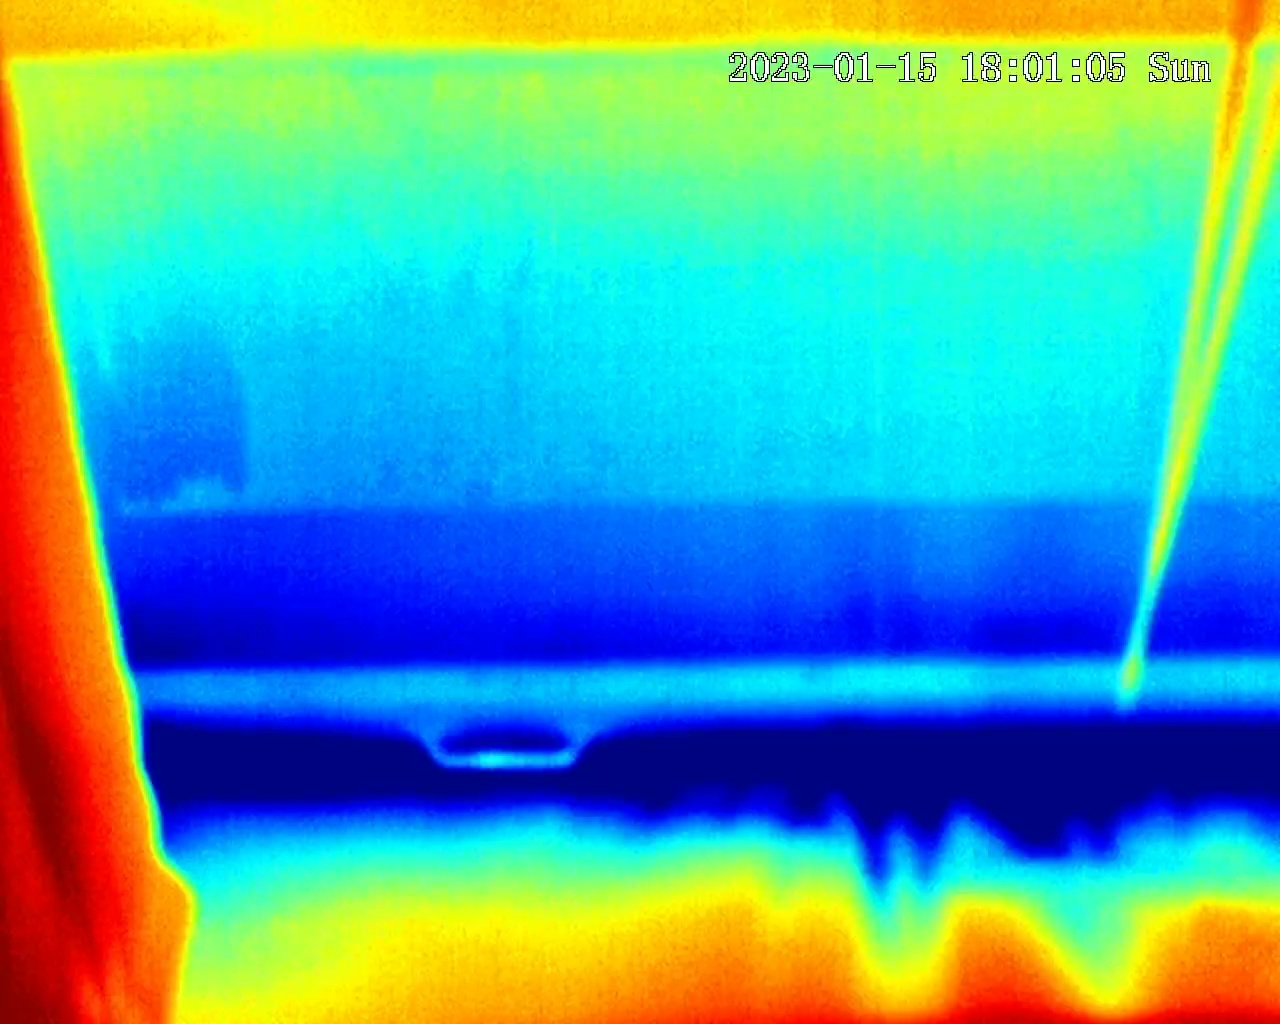
\includegraphics[width = 4cm]{image/chapter_2/tep_example}
				\caption{}
			\end{subfigure}
			\begin{subfigure}{.45\textwidth}
				\centering
				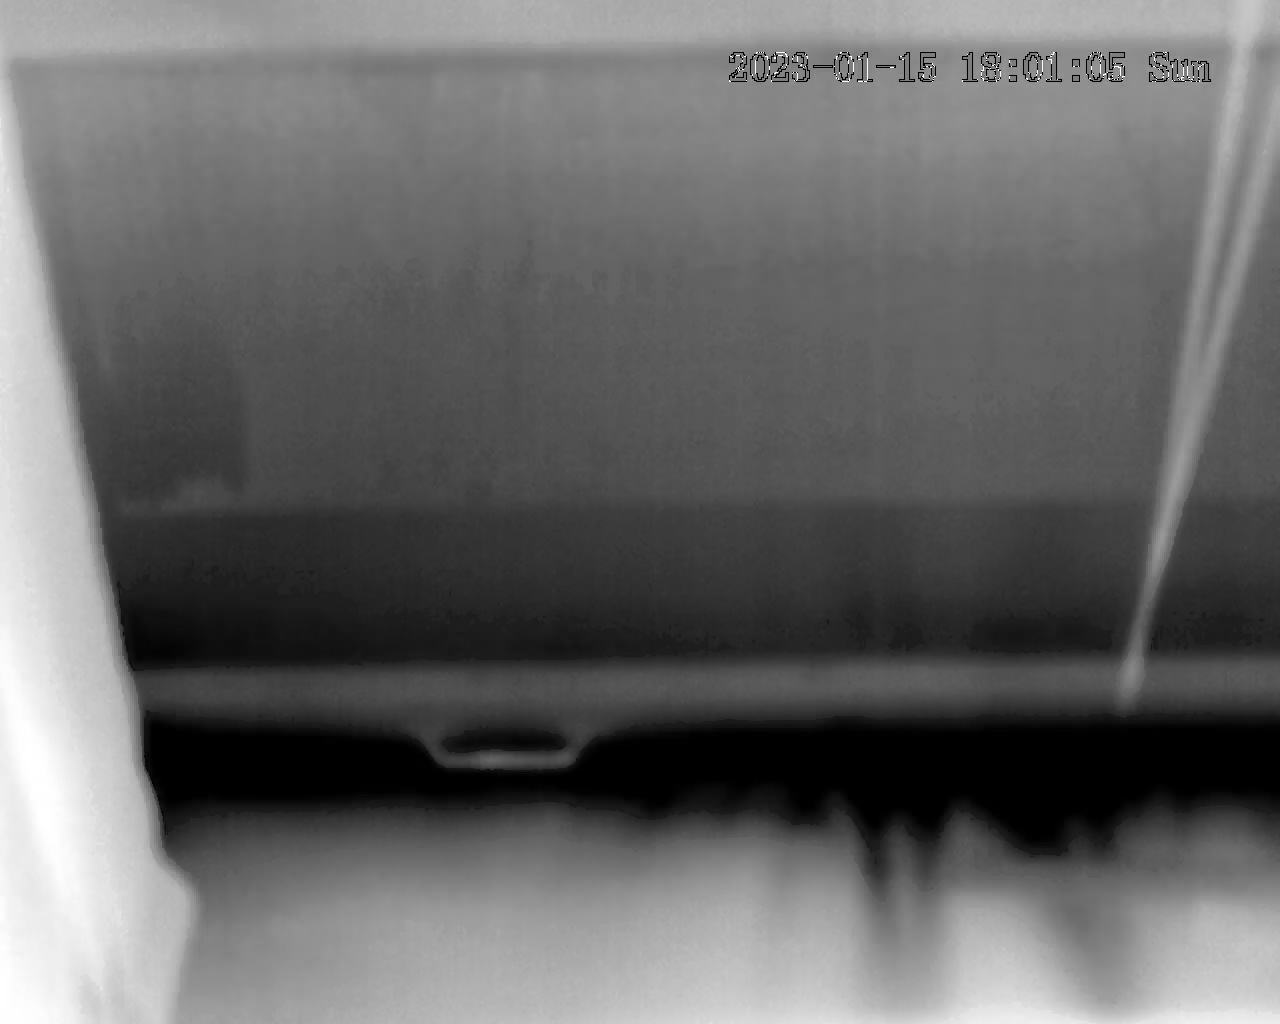
\includegraphics[width = 4cm]{image/chapter_2/gray_tep_example}
				\caption{}
			\end{subfigure}
			\centering
			\caption{Примеры преобразования цветовой карты, где (a) до; (б) после}
			\label{fig:ResKNN}
		\end{figure}
	\end{frame}

	\begin{frame}
		Для оценки точности была введена метрика, отражающая среднюю относительную разницу интенсивности пикселя:
		\begin{equation*}
			Acc = 1 - \frac{\sum\limits_{i=1}^h \sum\limits_{j=1}^w |P^{true}_{ij} - P^{conv}_{ij}|}{255wh},
			\label{eq:flanaccuracy}
		\end{equation*}
		где $w$ и $h$ -- размеры кадра. $P^{true}$ и $P^{conv}$ - некоторое изображение в оттенках серого и то же самое изображение, но с наложеной цветовой картой, сжатое с помощью JPEG и обработанное алгоритмом преобразования. В результате была получена точность 0,995777.
	\end{frame}

	\begin{frame}
		\bfseries Наложение карты абсолютных температур на оптические снимки. \normalfont
		
		Для преобразования карты относительных температур к абсолютным была использована формула:
		\begin{equation*}
			T_{abs} = T_{min} + \frac{T_{relative}(T_{max} - T_{min})}{255},
			\label{eq:Cjetgray}
		\end{equation*}
		\begin{figure}[h!]
			\centering
			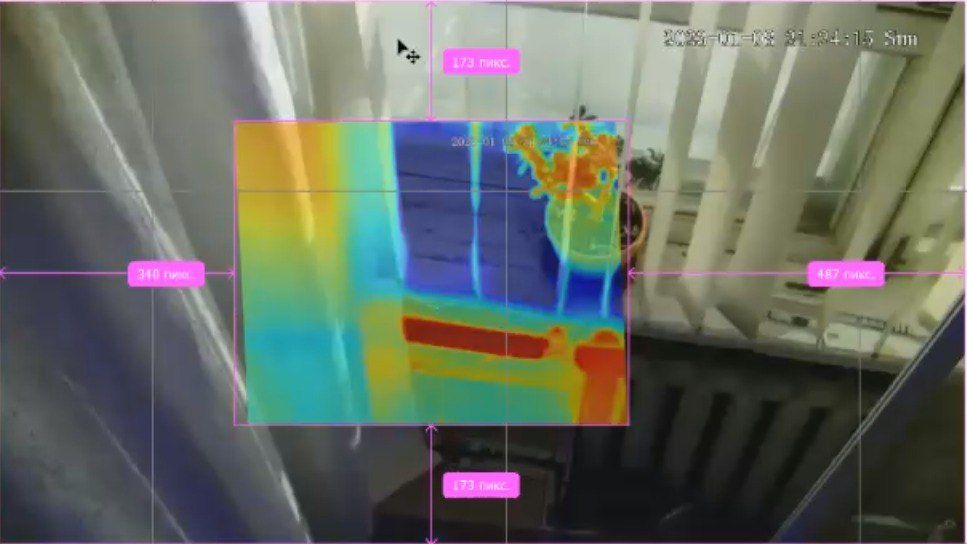
\includegraphics[width = 6cm]{image/tep+opt}	
			\caption{Наглядный пример наложения теплового снимка на оптический}
			\label{fig:tep+opt}
		\end{figure}
	\end{frame}

\section{Результаты}

	\begin{frame}
		На данный момент реализована сегментация по методу отсечения по пороговому значению. Порогом является медианная абсолютная температура.
		\begin{figure}[h!]
			\centering
			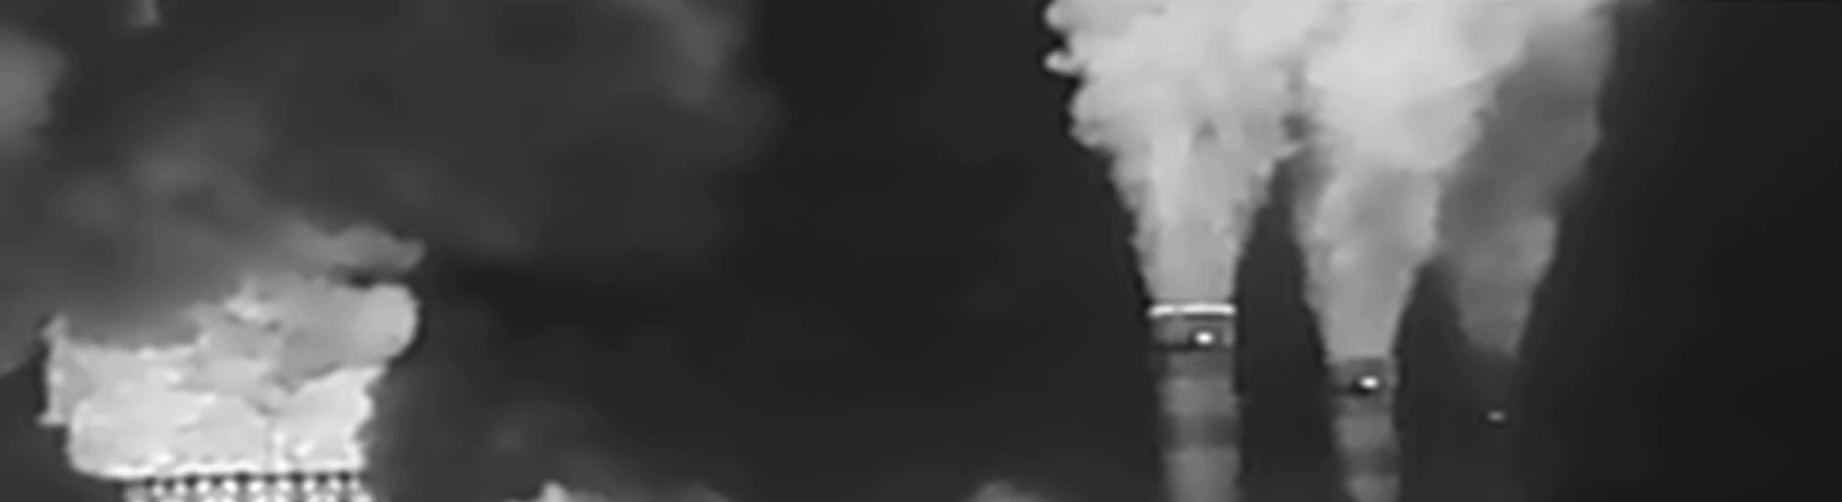
\includegraphics[width = 7cm]{image/img}	
			\caption{Изображение в оттенках серого}
			\label{fig:segbef}
		\end{figure}
		\begin{figure}[h!]
			\centering
			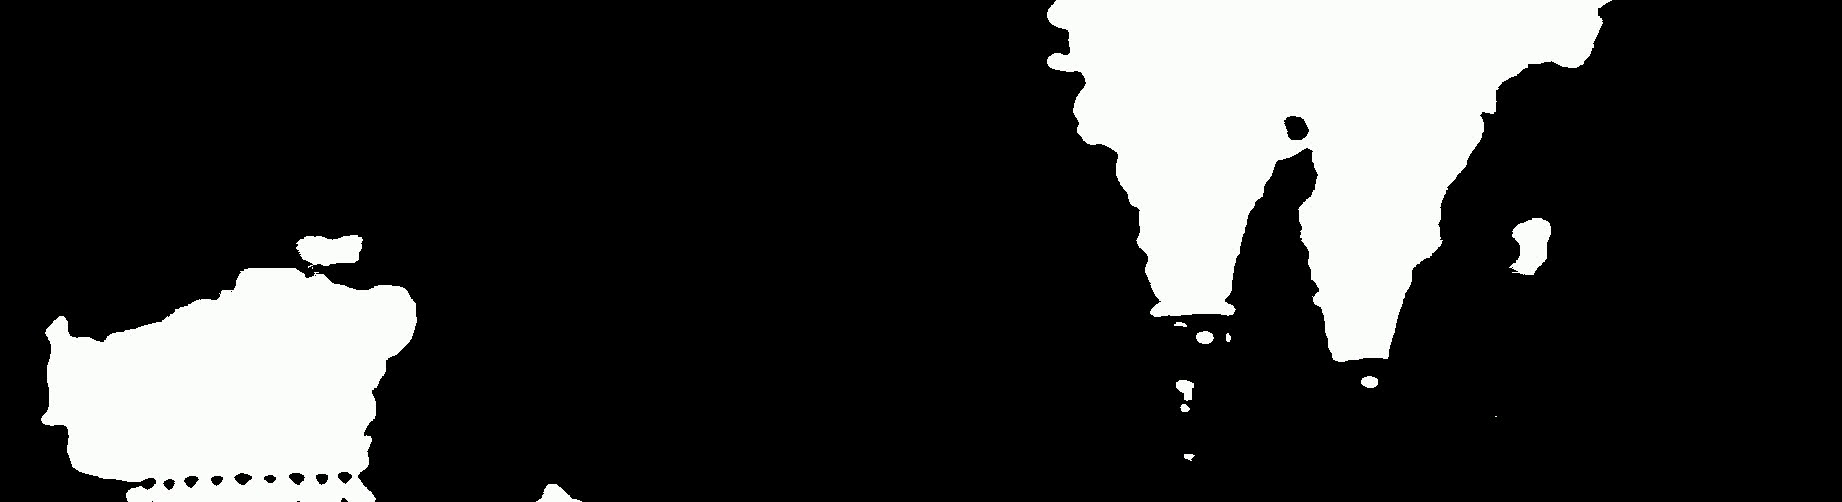
\includegraphics[width = 7cm]{image/seg}	
			\caption{Маска после сегментации}
			\label{fig:segaft}
		\end{figure}
	\end{frame}
	\begin{frame}
	\begin{center}
		\vspace{3cm}
		\Huge{Спасибо за внимание!}
	\end{center}
	\end{frame}

\end{document}
